\subsection{Network Density and Connectivity}\label{subsec:network-density-and-connectivity}
Even with the disconnected nodes removed, the graph appears to be extremely sparse.
This is apparent from the density, which  may be calculated as follows:
\[
    D = \frac{2E}{N(N - 1)}
\]

With 8574 nodes and 10790 edges, the density is $~0.00029$.
Considering that a graph's density is such that: ($0 \leq density \leq 1$), this graph is rather disconnected.

\subsection{Average Degree and Degree Distribution}\label{subsec:average-degree-and-degree-distribution}
The average node degree is 1.258, reinforcing the perception that the graph is sparse.
This low density may cause problems down the line, as link prediction methods commonly perform better on denser graphs

The degree distribution (figure~\ref{fig:degree-distribution})
shows that there are a few nodes in the graph that are exceedingly central
(upwards of 300 edges).
After some investigation,
it was found that these nodes generally correspond to large medieval cities or countries such as Baghdad,
Alexandria or Yemen.
Besides these highly central nodes, most nodes (6000+) only have a single edge.

\begin{figure}[h] % [h] attempts to place figure here, other options like [t]op, [b]ottom
    \centering % Centers the figure horizontally
    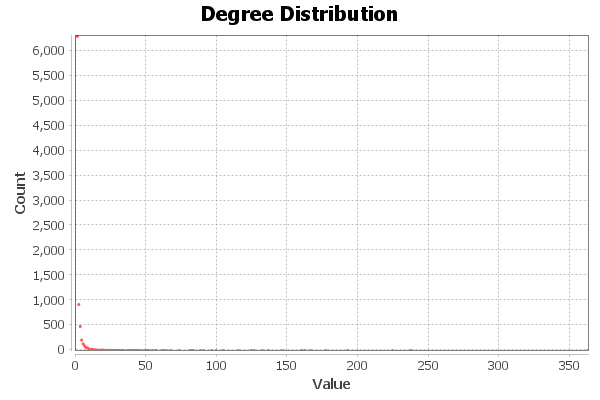
\includegraphics[width=1\linewidth]{figures/degree-distribution/degree-distribution} % Include the image with desired width
    \caption{Degree Distribution of the initial graph.} % Add a caption
    \label{fig:degree-distribution} % Assign a label for referencing the figure in text
\end{figure}


\subsection{Modularity}\label{subsec:modularity}
Using Gephi's~\cite{Gephi} implementation of the Louvian method~\cite{Louvian} with a resolution of 5.0,
217 communities were found.
However, the high number of communities is only indicative of a highly disconnected graph, with many small, isolated islands.
In practice, eight large groups account for 94.62\% of the nodes.
The modularity breakdown is shown on table:~\ref{tab:luv-communities}


\begin{table}[]
\centering
\begin{tabular}{|l|l|l|}
\hline
\textbf{Name} & \textbf{Population} & \textbf{Color on Figure ~\ref{fig:communities}} \\ \hline
Group 1       & 22.26\%             & Pink                     \\ \hline
Group 2       & 17.46\%             & Green                    \\ \hline
Group 3       & 15.13\%             & Blue                     \\ \hline
Group 4       & 9.41\%              & Black                    \\ \hline
Group 5       & 9\%                 & Orange                   \\ \hline
Group 6       & 8.69\%              & Red                      \\ \hline
Group 7       & 6.85\%                & Yellow                   \\ \hline
Group 8       & 5.82\%                & Cyan                     \\ \hline
\end{tabular}
\caption{Communities detected by the Louvain method}
\label{tab:luv-communities}
\end{table}

Figure~\ref{fig:communities} shows that the detected, large communities are fairly easy to visually distinguish.
Moreover, it shows that the highly central nodes (visualized by a larger diameter) are spread around the communities fairly evenly.

\begin{figure}[h] % [h] attempts to place figure here, other options like [t]op, [b]ottom
    \centering % Centers the figure horizontally
    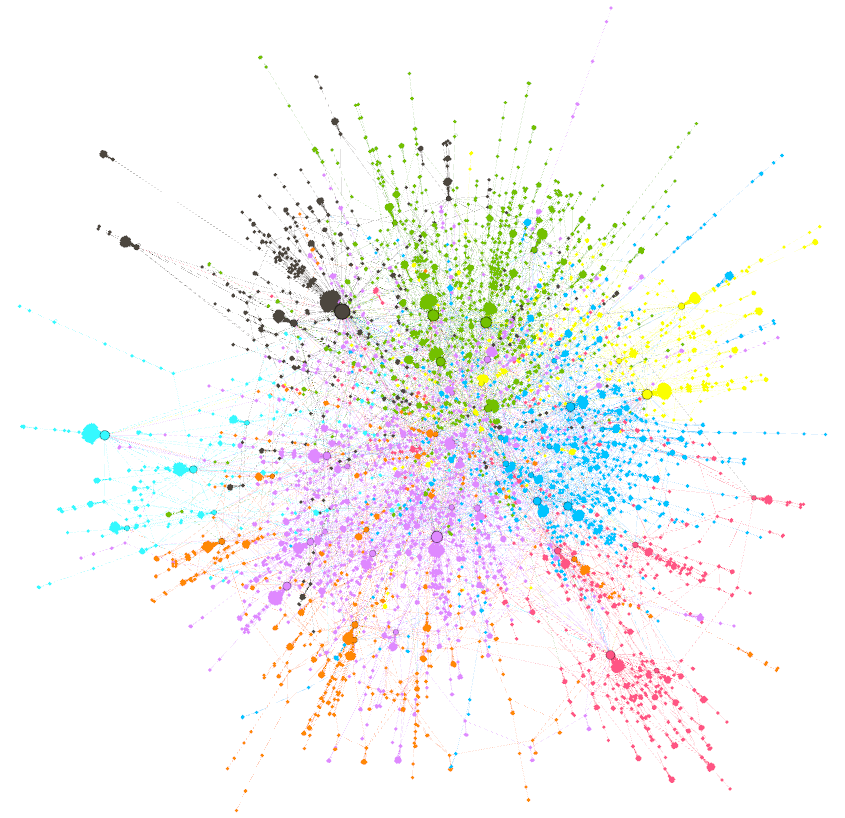
\includegraphics[width=0.7\linewidth]{figures/modules} % Include the image with desired width
    \caption{Graph visualization showing the communities listed on table~\ref{tab:luv-communities}} % Add a caption
    \label{fig:communities} % Assign a label for referencing the figure in text
\end{figure}.

\subsection{Unexpected Patterns}\label{subsec:odd-patterns}
While working with the parsed dataset, some odd patterns were found.
First, distance triplets were found, where both the head and tail entities were the same.
At the recommendation of the head, author of ~\cite{YaqutRB}, these triplets were discarded.

\begin{figure}[h] % [h] attempts to place figure here, other options like [t]op, [b]ottom
    \centering % Centers the figure horizontally
    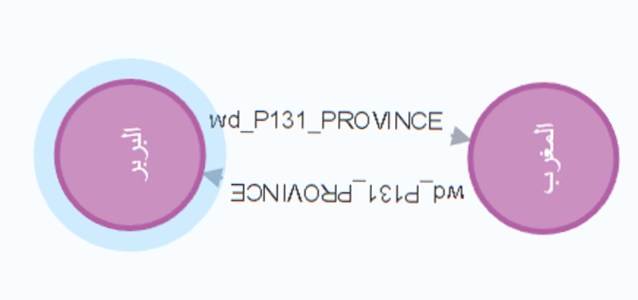
\includegraphics[width=0.5\linewidth]{figures/odd1} % Include the image with desired width
    \caption{Unusual hierarchical pattern where two nodes reference each other as their province.} % Add a caption
    \label{fig:odd1} % Assign a label for referencing the figure in text
\end{figure}

Secondly, during manual observation of the data, "odd" hierarchical patterns were observed;
that did not fit to the classical strict, unidirectional layout of other similar structures, shown on figure~\ref{fig:odd1} and ~\ref{fig:odd2} .

\begin{figure}[h] % [h] attempts to place figure here, other options like [t]op, [b]ottom
    \centering % Centers the figure horizontally
    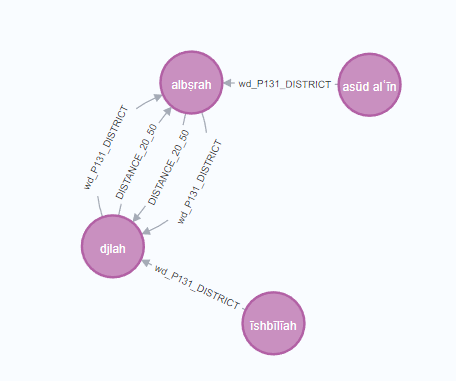
\includegraphics[width=0.5\linewidth]{figures/odd2} % Include the image with desired width
    \caption{Unusual hierarchical pattern where two nodes reference each other as their district.} % Add a caption
    \label{fig:odd2} % Assign a label for referencing the figure in text
\end{figure}

These patterns were extracted and forwarded to the MEHDIE researchers using the following Neo4J query:
\begin{verbatim}
    MATCH (n)-[:{r1}]->(m)-[:{r2}]->(n) RETURN n,m
\end{verbatim}

Where r1 and r2 correspond to all potential pairwise combinations of the edge types:
\textbf{wd\_P131\_METROPOLITAN}, \textbf{wd\_P131\_DISTRICT} and \textbf{wd\_P131\_PROVINCE}

